                                                                               \documentclass[tikz]{standalone}
\usepackage{lmodern}
\usepackage[algoruled,vlined,linesnumbered,titlenotnumbered,noend]{algorithm2e}
\usepackage{color,amsmath,bm,bbm,stmaryrd,amssymb,pifont,bbding}
\usetikzlibrary{backgrounds}
\usetikzlibrary{calc} 

\usetikzlibrary{shapes}
\usetikzlibrary{shadows}
\usetikzlibrary{decorations.pathmorphing}
\usetikzlibrary{decorations.text}
\usetikzlibrary{decorations}
\usetikzlibrary{arrows,bending}
\usetikzlibrary{shapes.arrows}
\tikzset{nobg/.style={show background rectangle,background rectangle/.style={opacity=0}}}


\input ../../styles
\input ../../globalcomm
\usetikzlibrary{arrows, shapes.gates.logic.US, calc}

  \tikzstyle{bddnode}=[draw,rectangle,rounded corners=2mm]
  \tikzstyle{aops}=[pos=0.9,below,yshift=0mm,xshift=-2mm]
\begin{document}
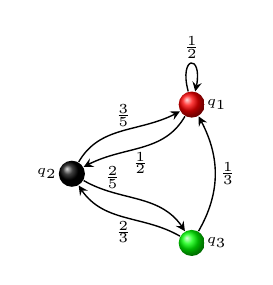
\begin{tikzpicture}
\node[circle, ball color=black,name=black]{};
\node[circle,ball color=red,name=red] at ($(black)+(30:50pt)$){};
\node[circle,ball color=green,name=green] at ($(black)+(-30:50pt)$){};

\draw[->,>=stealth,out=60,in=210,line width=0.5pt] (black) to 
node[font=\tiny,above=-2pt]{$\frac35$}
(red);
\draw[->,>=stealth,out=240,in=30,line width=0.5pt] (red) to 
node[font=\tiny,below=-2pt]{$\frac12$}
(black);
\draw[->,>=stealth,out=330,in=120,line width=0.5pt] (black) to 
node[font=\tiny,above=-2pt,near start]{$\frac25$}
(green);
\draw[->,>=stealth,out=150,in=300,line width=0.5pt] (green) to node[font=\tiny,below=-2pt]{$\frac23$}
(black);
\draw[->,>=stealth,out=60,in=300,line width=0.5pt] (green) to 
node[font=\tiny,right=-2pt]{$\frac13$}
(red);
\draw[->,loop above,>=stealth,line width=0.5pt] (red) to 
node[font=\tiny,above=-2pt]{$\frac12$}
(red);

\node[anchor=west,font=\tiny] at ($(red.east)+(-3pt,0pt)$) {$q_1$};
\node[anchor=east,font=\tiny] at ($(black.west)+(3pt,0pt)$) {$q_2$};
\node[anchor=west,font=\tiny] at ($(green.east)+(-3pt,0pt)$) {$q_3$};
\end{tikzpicture}


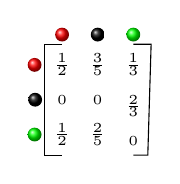
\begin{tikzpicture}
\node[font=\tiny,name=RR] at (0,0) {$\frac12$};
\node[font=\tiny,name=RB,anchor=north] at (RR.south) {$0$};
\node[font=\tiny,name=RG,anchor=north] at (RB.south) {$\frac12$};

\node[font=\tiny,name=BR,anchor=west] at (RR.east) {$\frac35$};
\node[font=\tiny,name=BB,anchor=north] at (BR.south) {$0$};
\node[font=\tiny,name=BG,anchor=north] at (BB.south) {$\frac25$};

\node[font=\tiny,name=GR,anchor=west] at (BR.east) {$\frac13$};
\node[font=\tiny,name=GB,anchor=north] at (GR.south) {$\frac23$};
\node[font=\tiny,name=GG,anchor=north] at (GB.south) {$0$};

\draw (RR.north) -- (RR.north west) -- (RG.south west) -- (RG.south);

\draw (GR.north) -- (GR.north east) -- (GG.south east) -- (GG.south);


\node[circle,inner sep=0pt, minimum size=5pt,outer sep=1pt, ball color=red,anchor=east] at ($(RR.west)$) {};
\node[circle,inner sep=0pt, minimum size=5pt,outer sep=1pt, ball color=black,anchor=east] at ($(RB.west)+(-1pt,0pt)$) {};
\node[circle,inner sep=0pt, minimum size=5pt,outer sep=1pt, ball color=green,anchor=east] at ($(RG.west)$) {};

\node[circle,inner sep=0pt, minimum size=5pt,outer sep=1pt, ball color=red,anchor=south] at ($(RR.north)$) {};
\node[circle,inner sep=0pt, minimum size=5pt,outer sep=1pt, ball color=black,anchor=south] at ($(BR.north)$) {};
\node[circle,inner sep=0pt, minimum size=5pt,outer sep=1pt, ball color=green,anchor=south] at ($(GR.north)$) {};


\end{tikzpicture}
\end{document}
